\chapter{Axelrod model for global polarization }

\resp{Marco Tavis Foster}


\section{Introduction}

    In this project we develop a model that explores cultural dissemination - with a specific focus on how nodes that have more similarities become more similar as they interact \cite{Axelrod1997}. Over the simulation we see distinct cultural clusters develop and global polarisation emerge where all global clusters are distinct enough where further interactions cannot occur - we reach dynamic stability. While clusters with completely different traits can no longer interact, local nodes that are similar will converge.

\section{Exploring a 10x10 grid}

    We first experiment with a 10x10 grid of 'villages' (represented by nodes) where each village has a number representing their culture. Each different digit in the number represents the number of cultural features each village has, and the different number a digit can take represents different cultural traits. The more features two neighbouring villages have in common the more similar their cultures are and the more likely they will interact to become more similar. We witness this setup in Fig. 1.1.

\begin{figure*}[t]
    \centering
    \begin{minipage}{0.49\textwidth}
        \centering
        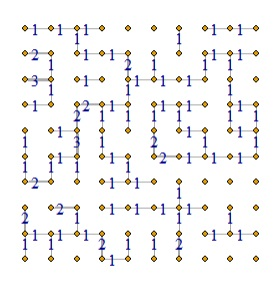
\includegraphics[width=\textwidth]{images/cultural_nodes1.jpg}
        \label{fig:sub1}
    \end{minipage}\hfill
    \begin{minipage}
{0.49\textwidth}
        \centering
        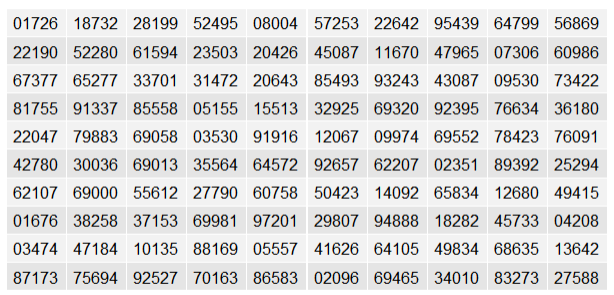
\includegraphics[width=\textwidth]{images/cultural_nodes2.jpg}
        \label{fig:sub2}
    \end{minipage}
    \caption{a) The 10x10 grid of 'villages'. The strength of the connection between villages represent how similar their cultures are. b) The cultural value of each village. In this example every village has 5 cultural features, each of which can have a trait of 0-9.}
    \label{fig:overall}
\end{figure*}

    Once the setup is created we can add dynamic cultural evolution to the system. For each timestep:
    
    1) A random village is selected and one of its neighbours is randomly selected too.
    
    2) The similarity of the culture of these two villages is determined (for how many features they have the same trait).
    
    3) A random number between 0 and 1 is determined and we check if it is smaller than the ratio of the number of shared features/number of total features.
    
    4) If it is smaller than this ratio then we select a random feature of the node's culture to gain the same trait as that of its neighbour - these two villages' culture becomes more similar.

    Under these rules we allow for cultures that are similar to become more similar, while cultures that share less features in common are less likely to become more similar.

\begin{figure}[t]
    \centering
    \begin{minipage}{0.45\textwidth}
        \centering
        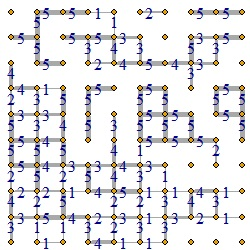
\includegraphics[width=\textwidth]{images/villagesEvol1.jpg}
        \caption{} % Subfigure label without numbering
        \label{fig:sub1}
    \end{minipage}\hfill
    \begin{minipage}{0.45\textwidth} % Adjusted width for second image
        \centering
        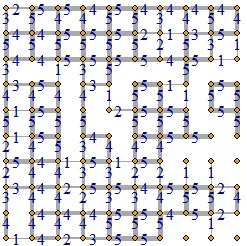
\includegraphics[width=\textwidth]{images/villagesEvol2.jpg}
        \caption{} % Subfigure label without numbering
        \label{fig:sub2}
    \end{minipage}
    
    \vspace{0.25cm} % Add some vertical space between rows
    
    \begin{minipage}{0.45\textwidth} % Adjusted width for third image
        \centering
        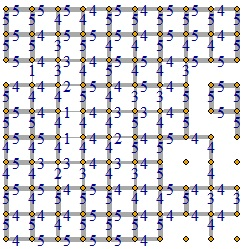
\includegraphics[width=\textwidth]{images/villagesEvol3.jpg}
        \caption{} % Subfigure label without numbering
        \label{fig:sub3}
    \end{minipage}\hfill
    \begin{minipage}{0.45\textwidth} % Adjusted width for fourth image
        \centering
        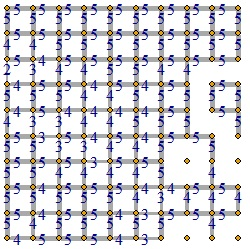
\includegraphics[width=\textwidth]{images/villagesEvol4.jpg}
        \caption{} % Subfigure label without numbering
        \label{fig:sub4}
    \end{minipage}
    
    \caption{The state of the system at timsteps: 1.2) t = 20,000. 1.3) t = 40,000. 1.4) t = 60,000. 1.5) t = 80,000}
    \label{fig:overall}
\end{figure}

    Observing Figures 1.2-5 we see how the system evolves over time. As the villages interact we see clusters of similar cultures emerge - by the end of the simulation we see that there is one large cluster of villages with the same/very similar cultures, along with  a cluster of 5 villages with the same culture and 4 villages that don't share a culture with any of their neighbours. 

    We repeat the simulation with different variables to test how the final system is different depending on changes to the initial parameters. I investigate varying the number of traits/features, the number of neighbours each village has, and the grid size. To compare differences in the final systems we will compare the number of stable regions - regions where all villages within it share cultural ties. In the last example (Fig 1.5) we observe 6 cultural regions for instance (4 of which are singular villages).

    Performing simulations when varying the number of features and number of traits per feature we get the data seen in Table 1.1. We note that increasing the number of traits increases the number of stable region, whilst doing the same with the number of features decreases it.  Adding more features provides more opportunities for villages to interact, whereas increasing the number of traits makes it more difficult for a given feature to be the same between neighbours.

\begin{table}[ht]
    \centering
    \begin{tabular}{c|ccc}
        Num Features (below), Num Traits (right) & 5 & 10 & 15  \\
        \hline
         5 & 1 & 2 & 5 \\
         10 & 1 & 1 & 1 \\
         15 & 1 & 1 & 1 \\
    \end{tabular}
    \caption{Simulations with varying number of traits and features per cultural value}
    \label{tab:my_label}
\end{table}

    We also run experiments where we alter the number of neighbours each village has. In order to visualise this better I changed the grid shape to be a 1D regular lattice where each village is connected to its k-nearest neighbours, where k is variable.  We see the results in Table 1.2. The data shows that as k increases the number of stable regions present at the end of the simulation decreases, which makes intuitive sense as the villages have more neighbours to interact with and so are more likely to adopt similar cultures

\begin{table}[ht]
    \centering
    \begin{tabular}{c|c}
    \hline
    k & Number of Stable Regions \\
    \hline
    1 & 10\\
    2 & 6\\
    3 & 3\\
    4 & 2\\
    5 & 2\\
    6 & 2\\
    7 & 3\\
    8 & 1\\
    9 & 1\\
    10 & 2\\
    \hline
    \end{tabular}
    \caption{Number of stable regions present as the number of neighbours k for each village changes}
    \label{tab:my_label}
\end{table}
    \centering

    Finally we experiment with increasing the number of villages in the system. We choose to utilise the same 1D lattice structure as it is simpler to add nodes to this structure. We fix k = 2, num-features = 5 and num-traits = 10. Results are shown in Table 1.3. We see that the number of stable regions increase with the number of villages as we expect. 

\begin{table}[ht]
    \centering
    \begin{tabular}{c|c}
        Number of Villages & Number of Stable Regions  \\
        \hline
         10 & 3 \\
         20 & 3\\
         30 & 9\\
         40 & 11\\
         50 & 10\\
         60 & 15\\
         70 & 19\\
         80 & 18\\
         90 & 21\\
         100 & 26\\
         110 & 22\\
         120 & 17\\
         130 & 32\\
         140 & 28\\
         150 & 34\\
    \end{tabular}
    \caption{Number of stable regions against the number of villages}
    \label{tab:my_label}
\end{table}
\newpage